%! TEX root = 'main.tex'
\section{Evaluation}
\label{sec:evaluation}

\begin{figure}[th]
	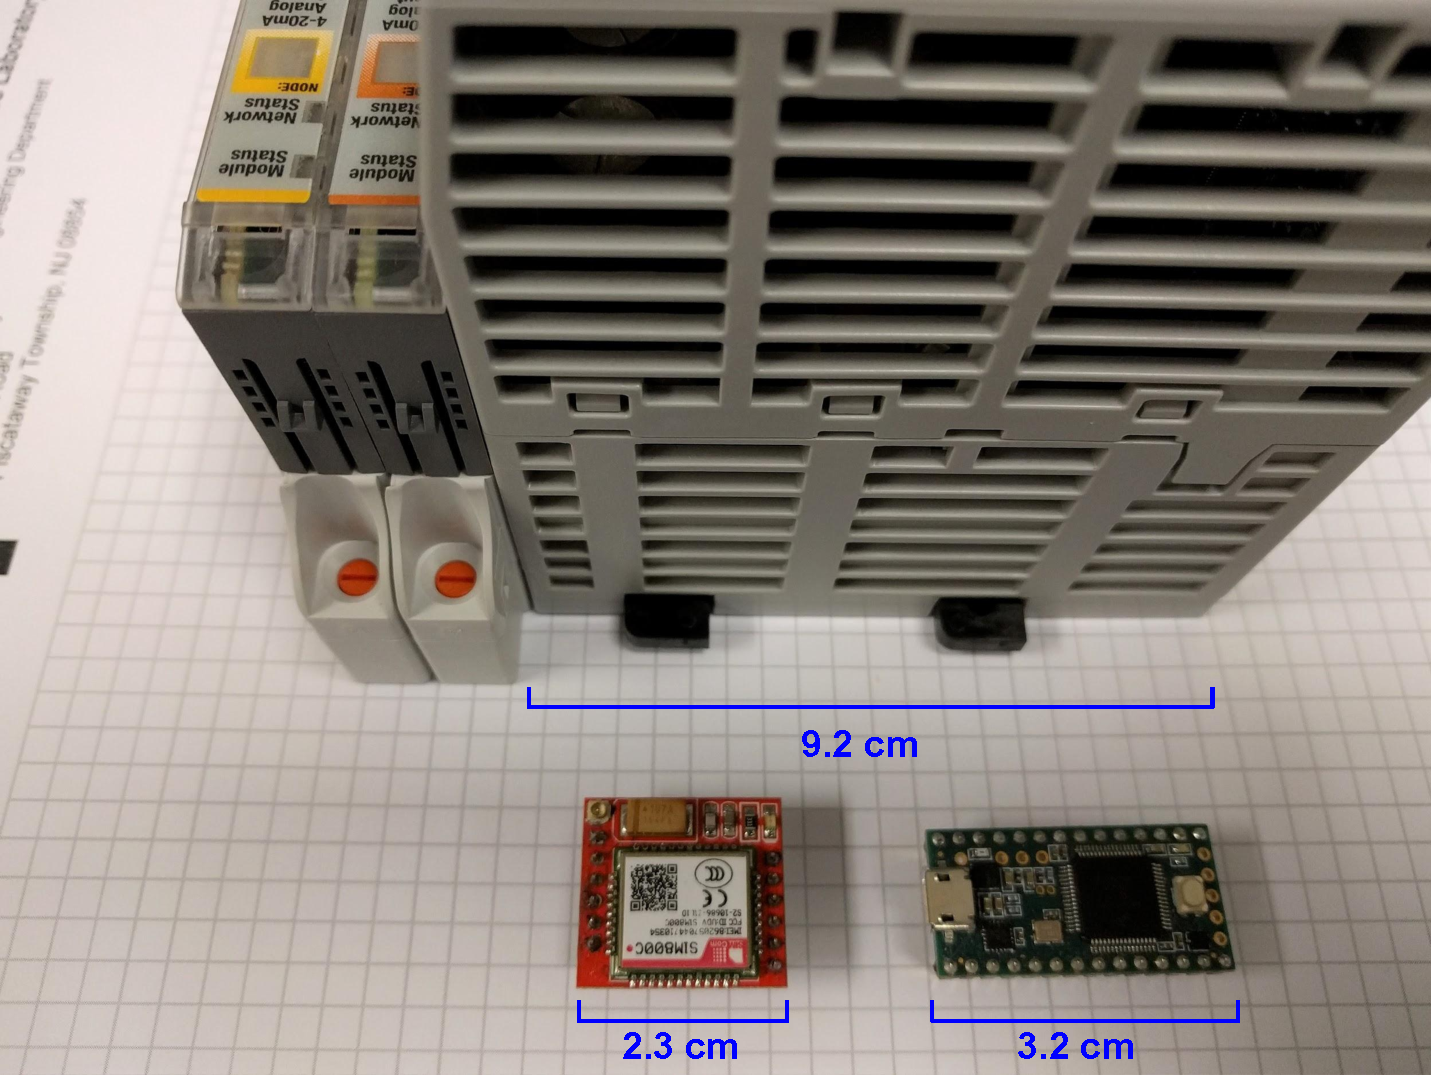
\includegraphics[width=0.47\textwidth]{figures/eval_size_old}
	\centering
	\caption{Test}
	\label{fig:eval_sizei_old}
\end{figure}

\begin{figure}[th]
	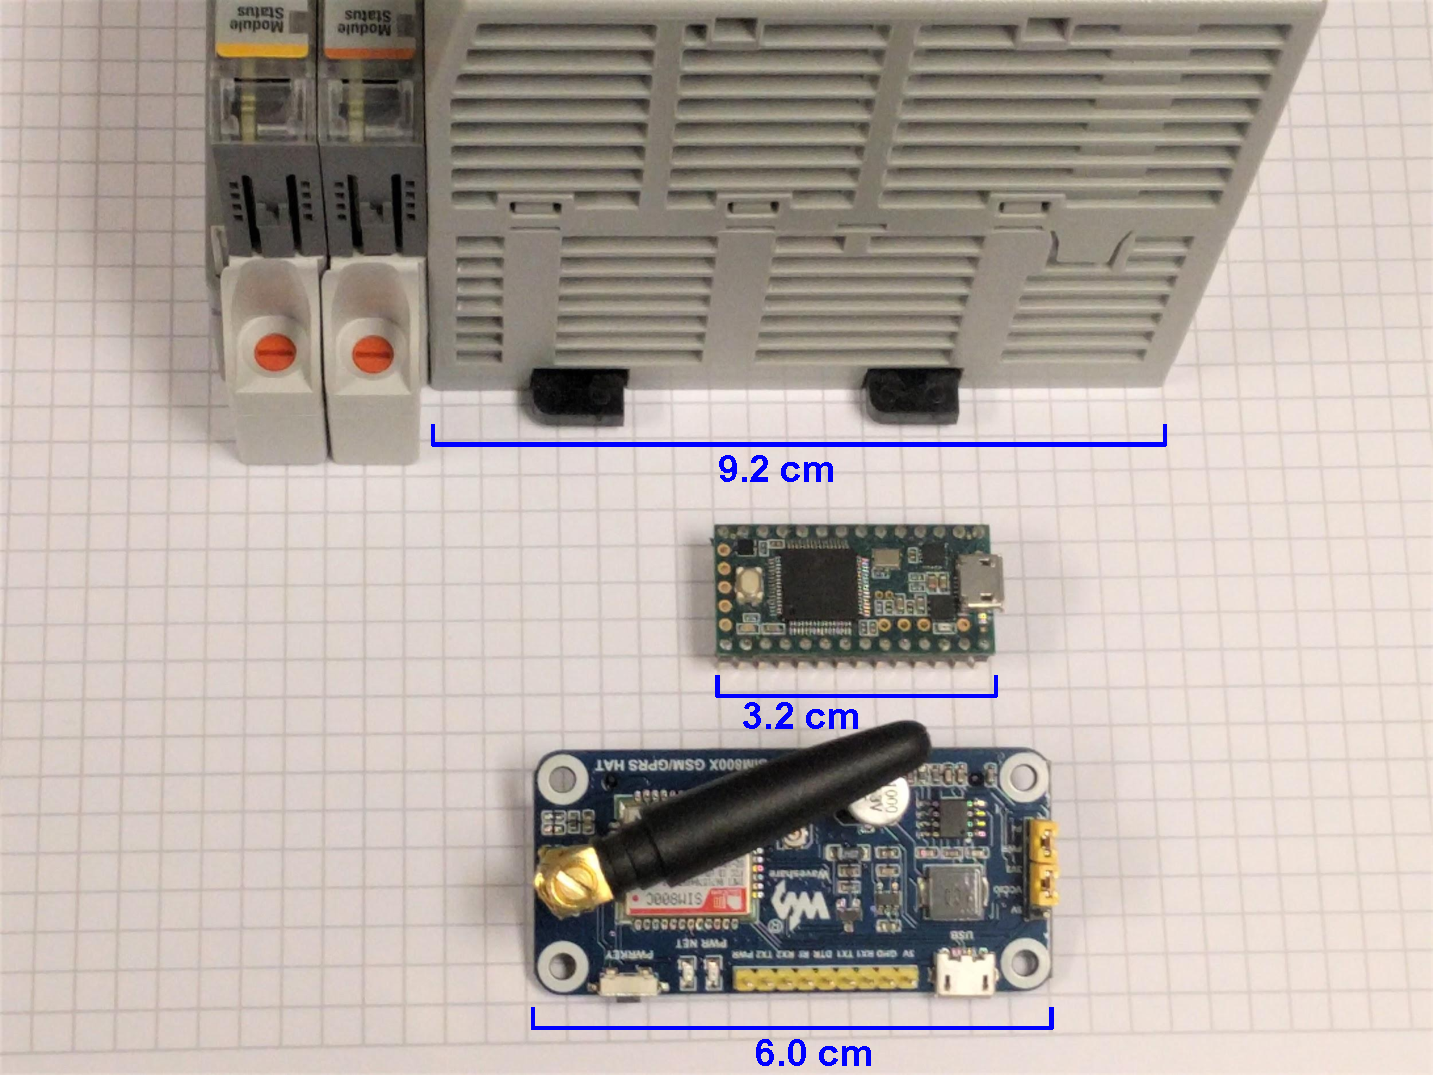
\includegraphics[width=0.47\textwidth]{figures/eval_size}
	\centering
	\caption{Test}
	\label{fig:eval_size}
\end{figure}


In our threat model, this hardware implant should exist independently of the PLC's communication network. To achieve this, as mentioned before, we chose to use cellular networks to communicate with nodes via SMS message. This approach is not as reliable as wired networks, especially in our attack model, which may require multiple nodes to launch attacks at the same time. We evaluated the approximate time required for SMS transmission, as shown in~\autoref{fig:smstime}, although we know that this may be affected by a variety of factors, such as the distance between the cell phone and the base station, the number of cell phones served by the same base station, across different networks, and so on. We also know that a SMS message over 160 characters will be split, large messages are segmented into 153 character segments and sent individually then rebuilt by the recipients device. But in order to avoid differences in the protocols implemented by different SMS programs or there may be some extra bytes attached to the SMS message, we did not strictly evaluate it by the number of SMS segments. From a practical point of view, we evaluated the transmission time corresponding to the length of the control command.

\begin{figure}[th]
	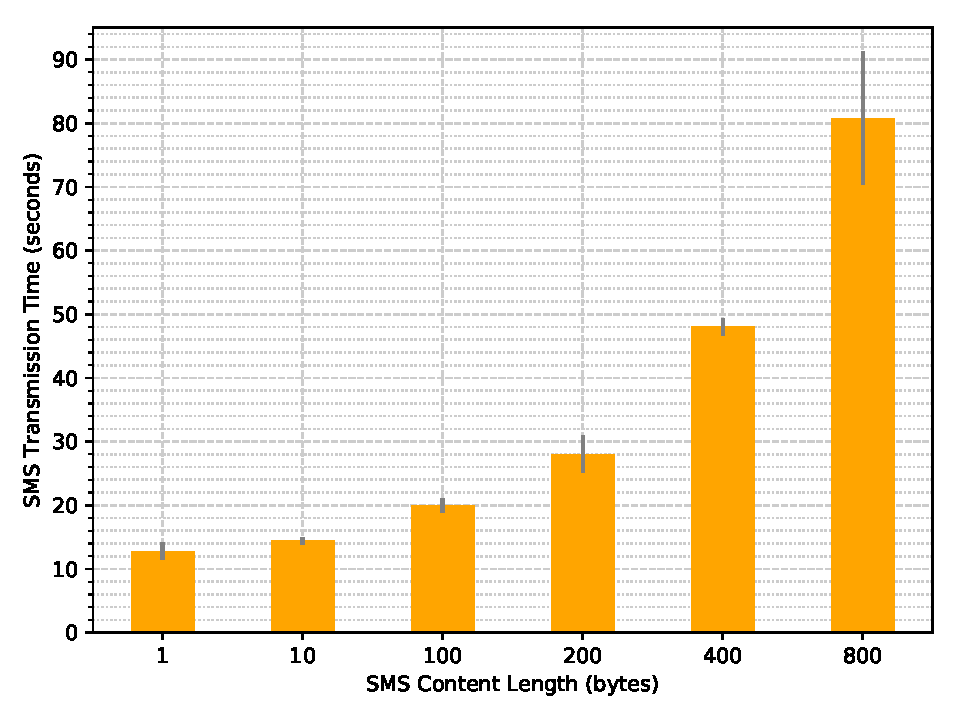
\includegraphics[width=0.47\textwidth]{figures/smstime}
	\centering
	\caption{SMS Message Transmission Time}
	\label{fig:smstime}
\end{figure}

The control command length can be only one byte, which is used to start a malicious function preset in the hardware implant. It can also be very long, such as containing a piece of binary to update the firmware of the PLC. Or it can contain a series of detailed attack instructions. The advantage of this is that even if the hardware implant is exposed, it does not contain specific attack instructions, thus avoiding further exposure to subsequence attacks and methods.

We get the data by sending a control command to a node with a phone. The command for each length was tested 20 times to obtain the mean and standard deviation. The cellular networks we used is T-Mobile and Google Fi. 

As shown in the figure, the longer the length of the control command, the more time it takes, and the less reliable it is for an attack that requires precise synchronization.

Since the payload (attack commands) is either pre-existing in the hardware implant or sent by the command message during the attack. The attack in our instance directly manipulates the output of the GPIO. So it does not need to modify any code in any PLC firmware, nor does it need to occupy the storage space of the PLC.

Due to different implementations, JTAG debugging capabilities can be intrusive or non-intrusive. The conventional JTAG debug is invasive which halt the processor using breakpoints and watchpoints. It also needs to halt the processor before it can modify any register. However, the debug functionality implemented in LM3S2793 is known as CoreSight architecture. The DAP (Debug Access Port) is an implementation of an ARM Debug Interface which provides real-time access for the debugger without halting the processor to AMBA system memory, peripheral registers and all debug configuration registers. So our hardware implant can modify the GPIO through AHB bus without any software overhead.

\begin{figure*}[h]
	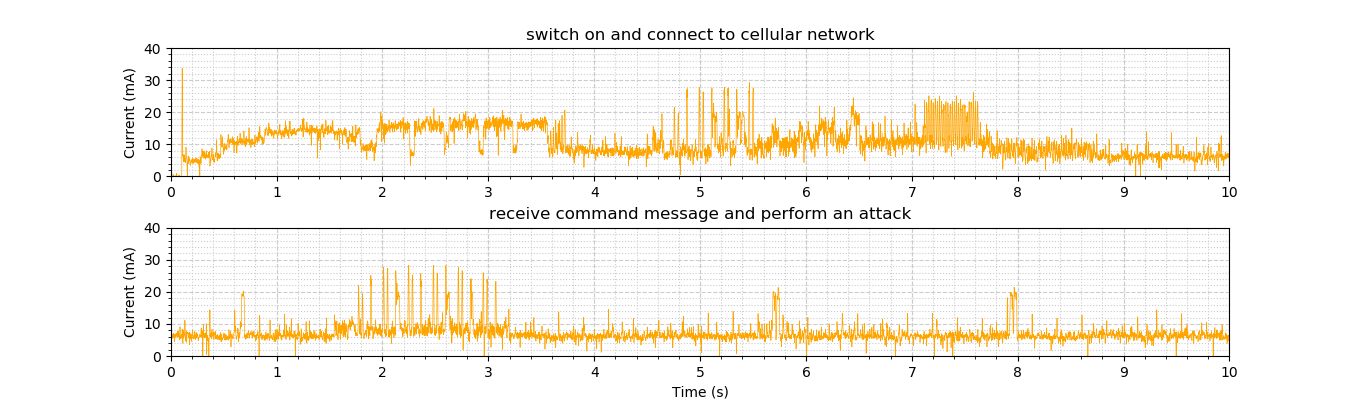
\includegraphics[width=\textwidth]{figures/current}
	\centering
	\caption{The hardware implant does not consume a lot of power, and the power consumption will only increase slightly when starting and executing the attack command. Sub-figure 1 shows the power consumption during the startup. Sub-figure 2.a shows the power consumption during an demo attack. 2.b indicates an output pin of the attacked PLC. }
	\label{fig:current}
\end{figure*}

The hardware implant is powered directly from the PLC and does not consume a lot of power. The power consumption will only increase slightly when starting and executing the attack command, as shown in~\autoref{fig:current}.



\subsection{Real-World Power System Case Study}

We evaluated the hardware implant on a real-world power system test-bed, where distributed PLCs with installed PID modules along with more complicated control algorithms (discussed below) maintain safe power system operation. 

The electricity grid is modeled using the mathematical power flow equations (physical Kirchhoff laws): 
\begin{equation}
\label{eq:powerflowreal}
f_i^p = -P_i^g+P_i^l + \sum_{k \in C}{|V_i||V_k| (G_{ik} \cos{\theta_{ik}} + B_{ik} \sin{\theta_{ik}}}),
\end{equation}
which mandate how the sensor measurements (e.g., real/reactive power values on $i$-th power node (bus) $P_i$/$Q_i$, power bus voltages $V_i$, inter-bus phase angles $\theta_{ij}$, and the admittance (inverse resistance) parameters ($G_{ij}, B_{ij}$) on the transmission line between the buses $i$ and $j$ correlate due to well-known physics Kirchhoff laws. $P_i^g$ represents the amount of power that is injected to the $i$-th power bus by a generator, and $P_i^l$ is the amount that is consumed by the end-users at that bus. 



\begin{figure*}[ht]
  \centering
  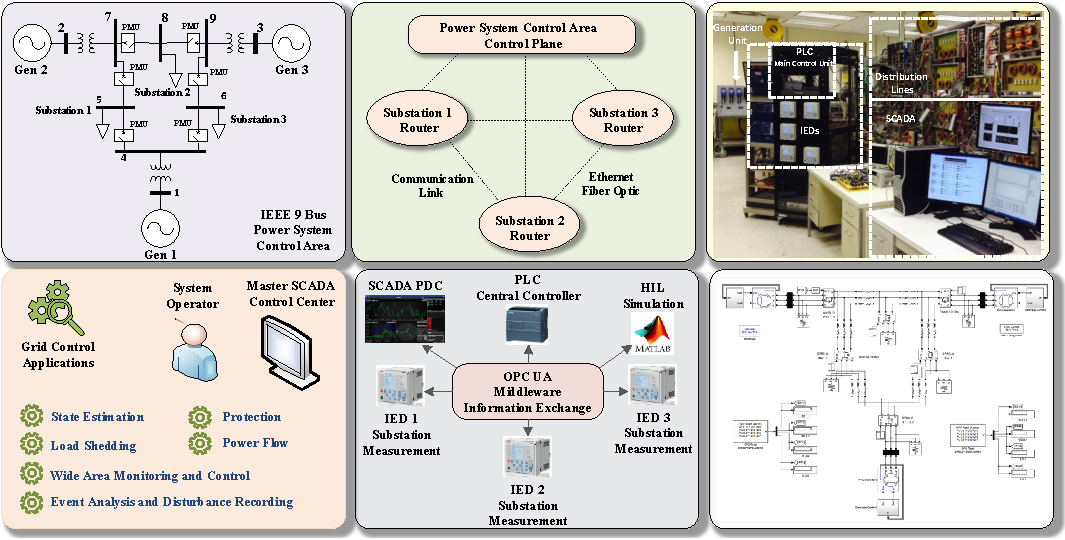
\includegraphics[width=0.85\textwidth]{figures/testbed2}
  \vspace{-0.0in}
  \caption{The Evaluation Smart Grid Test-Bed}
  \vspace{-0.1in}
  \label{fig:testbed}
\end{figure*}





Optimal power flow (OPF) is the most widely used control algorithm that is used in practice nowadays to calculate the optimal control commands continuously. In power systems, OPF finds an optimal power generation set-point that minimizes total cost $c$ while meeting operational safety constraints~\cite{FERCOPF}.  The control commands typically include power output (set-points) of generators~\cite{Tinney1968}. The OPF's equality constraints are the power balance equations at each bus in the system. Its inequality constraints are the network operating safety limits such as line flow capacities and generator power output limits:
\begin{equation} \label{eqn:opf}
\begin{aligned}
& \underset{u}{\min} & & c(x, u) \\
& \text{s.t.} & &  P_i^g - P_i^l = \sum_{k}{|V_i||V_k| (G_{ik} \cos{\theta_{ik}} + B_{ik} \sin{\theta_{ik}})} \\
& & &  Q_i^g - Q_i^l = \sum_{k \in C}{|V_i||V_k| (G_{ik} \sin{\theta_{ik}} - B_{ik} \cos{\theta_{ik}})} \\
%& & &   MVA_{ij} \leq MVA^{max}_{ij} \\
& & &  P_l^g \leq P^{gmax}_l\\
& & &  \forall i,j \in N, \; \forall l \in G, \; \forall k \in C \\
\end{aligned}
\end{equation} 
where $u$ denotes the controls commands to be calculated; $x$ represents dependent variables; $V$ and $\mathit{\theta}$ denote the bus voltage magnitudes and angles, respectively.


The legitimate OPF's objective is to minimize the cost while ensuring the system operates safely. The PLC hardware implant implements a modified version of the algorithm, malicious optimal power flow (mOPF), to maximize the cost without the need for compliance with safety constraints: 
\begin{equation} \label{eqn:opf1}
\begin{aligned}
& \underset{u}{\max} & & c(x, u) \\
& \text{s.t.} & &  P_i^g - P_i^l = \sum_{k}{|V_i||V_k| (G_{ik} \cos{\theta_{ik}} + B_{ik} \sin{\theta_{ik}})} \\
& & &  Q_i^g - Q_i^l = \sum_{k \in C}{|V_i||V_k| (G_{ik} \sin{\theta_{ik}} - B_{ik} \cos{\theta_{ik}})} \\
%& & &   MVA_{ij} \leq MVA^{max}_{ij} \\
%& & &  P_l^g \leq P^{gmax}_l\\
& & &  \forall i,j \in N, \; \forall l \in G, \; \forall k \in C \\
\end{aligned}
\end{equation} 
where the calculated control commands would \textit{maximize} the amount of possible damage to the power system. The calculated commands are used as set-points to be maintained by the inner-loop PID controllers. Please note that the specific objective function for different malicious goals can be simply used instead in the formulation above. 

Our power system test-bed implements IEEE nine-node (bus) benchmark topology~\cite{christie2000power} including three synchronous power generators and controlled by nine distributed PLCs. \Cref{fig:testbed} shows the test-bed (top right), its cyber network topology (top middle), power system topology (top left), Lab-View control diagram (bottom right), supervisory control and data acquisition device interconnections (bottom middle), and monitoring and control operations (bottom left). The model has three substations and corresponding loads (which consume power). The power nodes are connected through power transmission lines. To follow real world implementations, we equipped each substation with protection functions such as over-current, voltage and frequency, i.e., the substation will open a transmission line if they carry current beyond its physical capacity or cause over-voltage or over-frequency situations. To monitor the power system, the voltage and current sensors (phasor measurement units PMUs) send their measurements to PLC controllers that act as monitoring/control agents and are responsible for all operational functions in the system. 

On the cyber end, the testbed includes a human-machine interface (HMI) server to provide the system status to the operators through its connections to the PLC. The data exchange between different field devices is established by open platform communications (OPC) Client I/O servers~\cite{opc}. Kepware OPC Server provides embedded drivers to connect to the PLC. The testbed employs a ReLab device driver to connect to and obtain measurements (IEEE C37.118) from PMU sensors. Briefly, using Kepware’s IEC 61850 MMS clients, the KEPServerEX OPC Server drivers create an interface for any of the OPC clients running in the network. 

We evaluated the hardware implant for two attack scenarios. 

\noindent\textbf{Steady-state system malicious attack:} Repeated heavy load circuit breaker open/close triggering without loss of power system stability. In this scenario, the malicious PLC firmware randomly (blindly) selects a circuit breaker to attack and triggers the opening/closing of the breaker several times, i.e., a transmission line opened and closed repeatedly. The power system was able to withstand this attack scenario without losing the stability since the target circuit breaker load was in the limits of power system generation reserve capacity. The SEL-451 PMU is located on generator 1 bus, and the 421-PMU is located at generator 2 bus. \Cref{fig:attack1} shows the power system status during the attack that starts at 11.29.30 PM. The circuit breaker was opened and closed three times sequentially within ten seconds. The heavy loading in the system deteriorated the system frequency (\Cref{fig:attack1-1}) and voltage (\Cref{fig:attack1-2}). The AC phase angle difference between generator 1 and generator 2 exceeded permissible limits (\Cref{fig:attack1-3}). The power flow magnitudes (\Cref{fig:attack1-5}) also violated safety thresholds temporarily. As shown, although the instant voltage and frequency of the system exceeded permissible limits, the power system was able to withstand this type of attack. During the attack, the hardware implant was able to run the power system model on the PLC in parallel and generate fake legitimate-looking sensor measurements to be viewed by the operators. \Cref{fig:attack1-fake} shows the results (before the noise was added for the presentation clarity). As the attack on the physical plant would result in noticeable side effects such as equipment operational noise, it's outputs show a minor system perturbation within safety limits that is normally observed on daily dynamic power system operations. From the operators' viewpoint, the system acts safely and no corrective action is needed.


\begin{figure*}[tp]
	\centering
    \begin{subfigure}[b]{0.42\textwidth}
    	\centering
	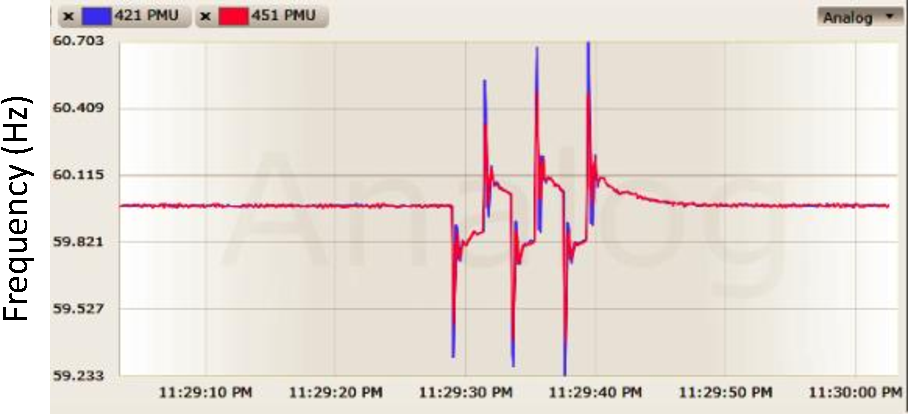
\includegraphics[width=1\textwidth]{figures/attack1-1}
        \vspace{-0.15in}
        \caption{Frequency}
		\label{fig:attack1-1}
	\end{subfigure}
~\qquad
	\begin{subfigure}[b]{0.42\textwidth}
    	\centering
	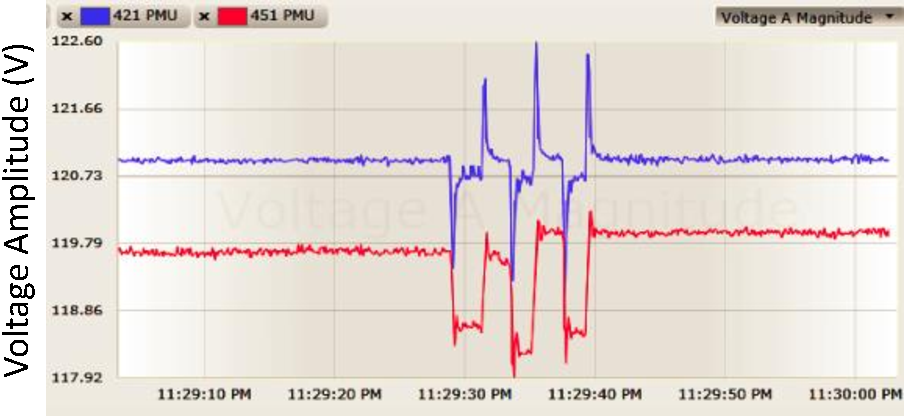
\includegraphics[width=1\textwidth]{figures/attack1-2}
        \vspace{-0.15in}
        \caption{Voltage Magnitude}
		\label{fig:attack1-2}
	\end{subfigure}
%~
	\begin{subfigure}[b]{0.42\textwidth}
    	\centering
	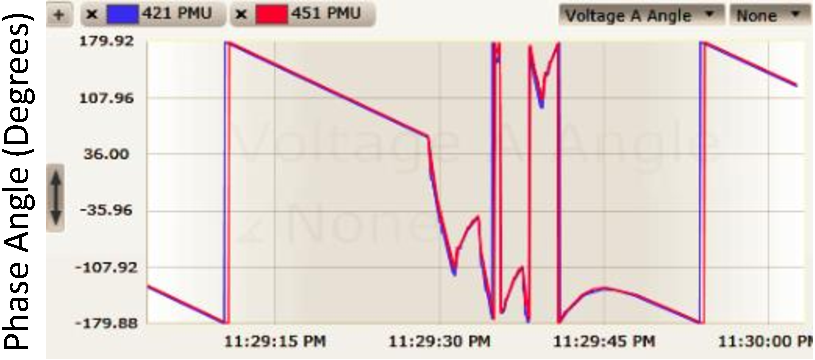
\includegraphics[width=1\textwidth]{figures/attack1-3}
        \vspace{-0.15in}
        \caption{AC Voltage Phase Angle}
		\label{fig:attack1-3}
	\end{subfigure}
~\qquad
	\begin{subfigure}[b]{0.42\textwidth}
    	\centering
	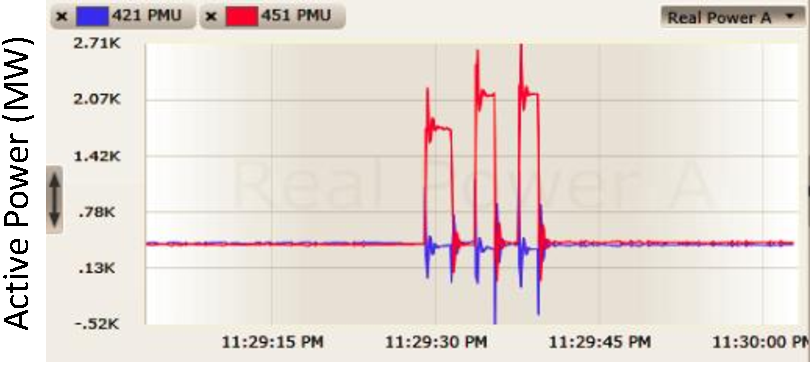
\includegraphics[width=1\textwidth]{figures/attack1-5}
        \vspace{-0.15in}
        \caption{Power}
		\label{fig:attack1-5}
	\end{subfigure}
    \vspace{-0.15in}
	\caption{Actual Power System Measurements}
	\vspace{-0.15in}
    \label{fig:attack1}
\end{figure*}

\begin{figure}[tp]
  \centering
  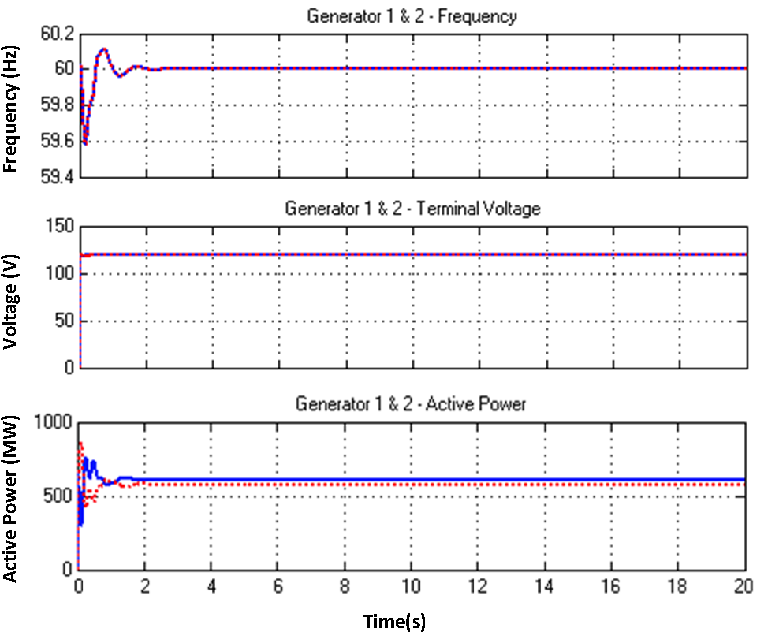
\includegraphics[width=.47\textwidth]{figures/attack1-fake}
  \vspace{-0.1in}
  \caption{Fake Measurements to Mislead the Operator}
  \vspace{-0.25in}
  \label{fig:attack1-fake}
\end{figure}


\noindent\textbf{Adversary-optimal control attack:} optimal malicious attack using real-world control algorithms. In this attack scenario, we implements a real-world power system controller algorithm, called optimal power flow (OPF)~\cite{bose2015equivalent}, that is widely used in power system control centers internationally. OPF is implemented as a linear programming function: it typically finds the optimal power system control strategy that minimizes the overall cost while ensuring the system safety. The system safety is usually defined by a set of lower and upper bound thresholds for various system parameters such as power transmission line current capacities, and minimum/maximum allowed system frequency 59.5-61Hz (60Hz is the nominal power grid frequency in USA). The control strategy is essentially a set of control commands that the PLC sends to the actuators, e.g., generation set-points to the generators that mandate how much power each generator should generate. The hardware implant implements the same control algorithm on the PLC after making three modifications to the algorithm (we call it malicious OPF - mOPF): \textit{i)} it removes the condition that ensures the system is within safety margins; \textit{ii)} it replaces the cost minimization function with maximization so that the adversarial impact becomes maximum; and \textit{iii)} the hardware implant adds predefined stealthy conditions to ensure its malicious control actions do not get noticed/detected by the local operators on site due to the noise the actions generate. Example conditions are ``no power generator disconnect from the rest of the power grid'' in large power plants, since such disconnects cause a noticeable sound noise to the potential local operators. In practice, there are typically few or no operators present on remote power system substations. This gives the hardware implant more freedom in terms of what malicious actions it can carry out. 

In this attack scenario, the hardware implant's objective was to implement mOPF on the PLC to calculate adversary-optimal control strategy for the power plant. Using the power system's safety constraints, the hardware implant intercepts the legitimate control action outputs and instead sends out its optimally-calculated malicious control commands to the power actuators at specific time points. The hardware implant sets the nominal frequency reference to 62 Hz, and its malicious controller calculates and sends out control commands accordingly.  

\begin{figure*}[tp]
	\centering
    \begin{subfigure}[b]{0.42\textwidth}
    	\centering
	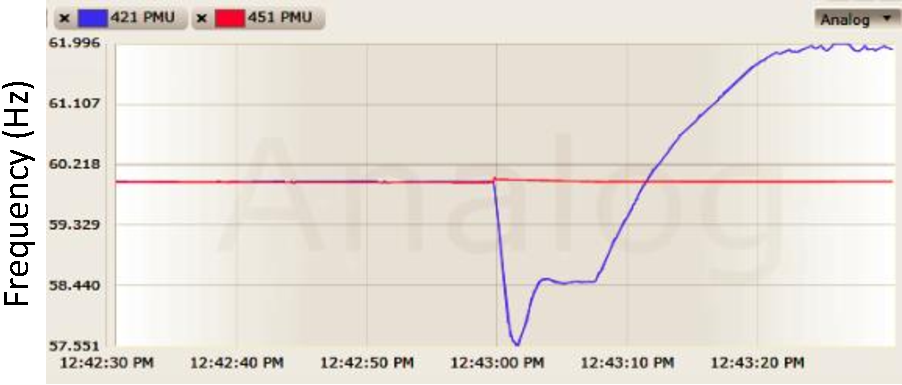
\includegraphics[width=1\textwidth]{figures/attack2-1-1}
        \vspace{-0.15in}
        \caption{Frequency}
		\label{fig:attack2-1}
	\end{subfigure}
~\qquad
	\begin{subfigure}[b]{0.42\textwidth}
    	\centering
	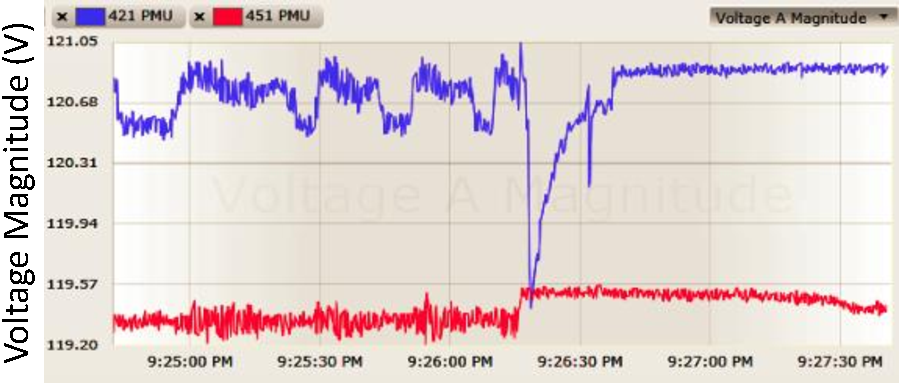
\includegraphics[width=1\textwidth]{figures/attack2-2}
        \vspace{-0.15in}
        \caption{Voltage Magnitude}
		\label{fig:attack2-2}
	\end{subfigure}
%~
	\begin{subfigure}[b]{0.42\textwidth}
    	\centering
	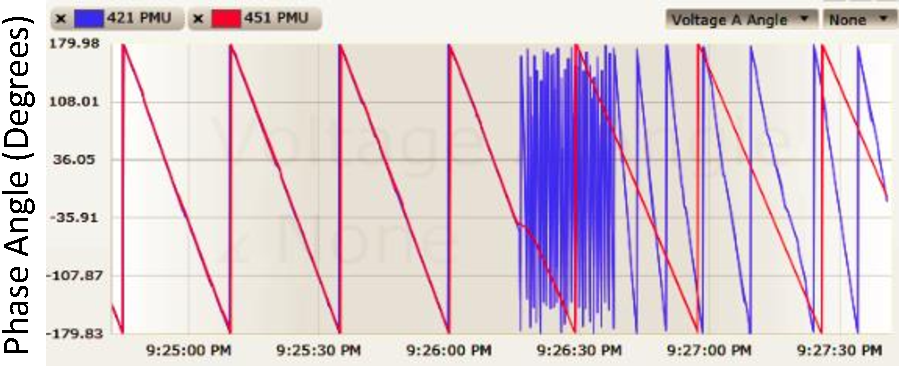
\includegraphics[width=1\textwidth]{figures/attack2-3}
        \vspace{-0.15in}
        \caption{AC Voltage Phase Angle}
		\label{fig:attack2-3}
	\end{subfigure}
~ \qquad
	\begin{subfigure}[b]{0.42\textwidth}
    	\centering
	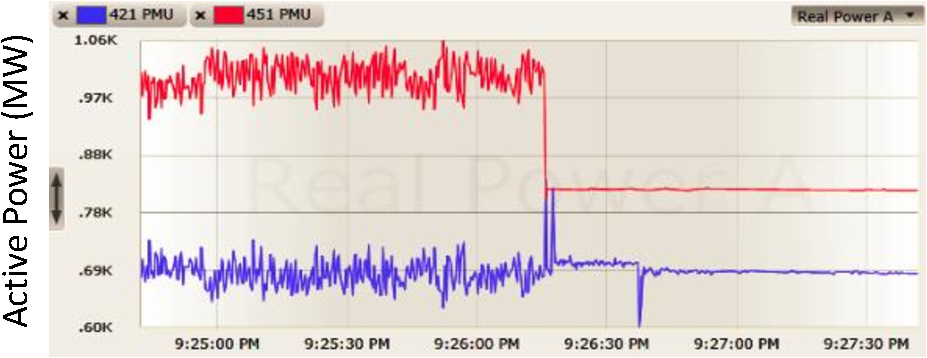
\includegraphics[width=1\textwidth]{figures/attack2-5}
        \vspace{-0.15in}
        \caption{Power}
		\label{fig:attack2-5}
	\end{subfigure}
    \vspace{-0.15in}
	\caption{Actual Power System Measurements}
    \vspace{-0.15in}
    \label{fig:attack2}
\end{figure*}

\Cref{fig:attack2} shows the actual power system measurements. The hardware implant makes the power system frequency exceed its safety margins through its malicious commands (\Cref{fig:attack2-1}). The system's voltage magnitude (\Cref{fig:attack2-2}), AC voltage phase angle (\Cref{fig:attack2-3}), and electric power values (\Cref{fig:attack2-5}) experience serious instability as well. However, in order to mislead the operator, the hardware implant implements a legitimate OPF algorithm in the background to simulate the power system and calculate individual system parameters assuming that the legitimate OPF control commands were carried out on the power system. The fabricated fake sensor measurements (\Cref{fig:attack2-fake}) are sent back to the operators' HMI screens. Consequently, from the operators' viewpoint, the underlying power system follows their expectation, while in reality, the system goes through serious instability situations facing potential large-scale failures.
An experienced operator might get suspicious of small disturbances visible in the graph.
However, such disturbances can also occur in normal operation.
Similarly, an automated tool monitoring the ICS must be tolerant to small disturbances to reduce the number of false positive alarms.

\begin{figure}[tp]
  \centering
  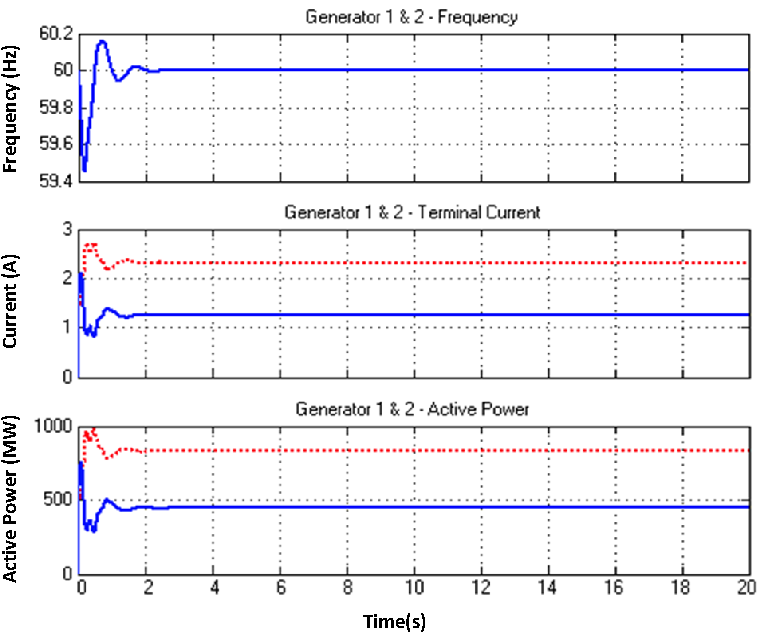
\includegraphics[width=.47\textwidth]{figures/attack2-fake}
  %\vspace{-0.15in}
  \caption{Fake Measurements to Mislead the Operator}
  \vspace{-0.3in}
  \label{fig:attack2-fake}
\end{figure}


